% --------------------------------------------------------------------



\section{Introduction}
\begin{sloppypar}
    In recent years the mobile app has revolutionized our daily lives. 
    These services have infiltrated social life, shopping and almost 
    every aspect of our existence. The services and their apps compete of 
    our time and markets are reinventing themselves constantly. The rapid 
    expansion and at times even faster decline of these web services 
    need a matching architecture to meet these very specific needs. 
\end{sloppypar}
\begin{sloppypar}
    There are many web services already in use which have been designed and 
    implemented before the onslaugh of microservices. Some of these services 
    need to evolve to be of use in the future. In many cases the monolith 
    services have already started to use certain aspects from the microservice 
    world, such as access tokens and REST API:s. The pressure from new 
    competitors adopting new technologies right from the start and the fact 
    that the industry and its developer base are extremely young dictates that 
    the old and established services have to address the situation someway or 
    the other. Monoliths have served us well but the time has come to evolve 
    with the customer needs.
\end{sloppypar}
\begin{sloppypar}
    Stackoverflow annual survey \citep{stackoverflowsurvey2019} conducted on 
    developers finds that half of the respondents identified as full-stack or 
    backend developers. The professional developers had very little experience 
    and about 40\% of them had less than five years of professional experience. 
\end{sloppypar}
\begin{sloppypar}
    The new developers entering the work force have very different mindset than 
    the older more seasoned professionals. Thus, it is very clear that the ways 
    of working and paradigms to be used are in constant change. The old and 
    established have to embrace the change and refactor their architecture 
    before it is too late. Microservices are not the proper choice for all needs
     \citep{newman2019} but in many cases there simply is no other valid choice.
    This change needs to happen in an orderly and safe way and the security 
    aspects need to be addressed. 
\end{sloppypar}
\begin{sloppypar}
    Microservice Architecture (MSA) differs in many ways from 
    the more tradition Monolith Architecture (MA). This shift entails very 
    specific security issues.
\end{sloppypar}
\begin{sloppypar}
    In this thesis the MSA and security literature is evaluated and the main 
    differences between MA and MSA on back end security aspects are found.
\end{sloppypar}
\begin{sloppypar}
    Chapter 2. presents the definitions used in this thesis. 
    Chapter 3. discusses the Confidentiality aspect of a switch from MA to MSA. 
    In chapter 4. Integrity of the information is discussed in the context of 
    MA and MSA. 
    Chapter 5. presents Availability when changing from MA to MSA.
    In Chapter 6. other relevat security aspects are presented.
    Chapter 7. contains the conclusions and presents further research topics.
\end{sloppypar}

\section{Definitions}
\begin{sloppypar}
    This thesis uses the following definitions.
\end{sloppypar}



\subsection{Microservice}
\begin{sloppypar}
    Microservice architecture can be viewed as an extension of the service oriented 
    architecture (SOA)\citep{newman2019,fowlerlewisms}. It's guiding principles are stated in the SOA manifesto 
    \citep{soamanifesto} and one is to prioritize:
    \begin{quotation}
        \noindent \it
        \begin{itemize}
            \item Business value over technical strategy
            \item Strategic goals over project-specific benefits 
            \item Intrinsic interoperability over custom integration 
            \item Shared services over specific-purpose implementations 
            \item Flexibility over optimization 
            \item Evolutionary refinement over pursuit of initial perfection
        \end{itemize}
    \end{quotation}
\end{sloppypar}
\begin{sloppypar}
    A microservice is a service that: is independently deployable,
    is modeled around business domain,
    that owns the data that they need to operate,
    that communicates via network,
    is technology agnostic,
    that encapsulates data storage and retrieval and 
    that has stable interface \citep{newman2019}.
\end{sloppypar}

\subsection{Security}
\begin{sloppypar}
    Security can be defined in multiple ways but in this thesis security 
    and more specifically information security is defined as consisting of 
    Confidentiality, Integrity, and Availability (CIA) as is stated in the 
    pocket book on ISO/IEC 27001 -standard for information security \citep{isoiec27001}.
\end{sloppypar}
\begin{sloppypar}
    The ISO/IEC 27001 standard defines confidentiality as such that information 
    or property is available to the authorized user only. The authorized users 
    can consist of persons, processes or entities to whom the information or 
    property can be disclosed. Integrity means that the data or property is 
    safeguarded for accuracy and completeness. Availability in this web service
    context is defined as such that the property or information is available 
    when it is needed.
\end{sloppypar}

\section{The Switch of Architectures}
\begin{sloppypar}
    To change the architecture from MA to MSA should be a gradual process. The 
    MA is or at least should be  split to modules with separation of concerns 
    \citep{secchalmsa}. The actual splitting of the monolith can be carried out
     in various ways. One of whic is DDD (SOURCE FOR THIS).
\end{sloppypar}

\begin{sloppypar}
    The MSA differs from a MA in fundamental ways. According to \citet{fowlerlewisms} 
    one of which is the communication between its components. In a monolith 
    application the processes can send function calls or method invocations 
    amongst them selves. In MSA the messaging is based on sending messages or 
    HTTP requests.
\end{sloppypar}

\begin{sloppypar}
    Function calls entail a stackframe creation in the call stack, execution of 
    the function code and finally popping the stackframe and returning the result. 
    The actual overhead depends on the language and systems used to run the 
    application (SOURCE). Compilers can optimize the code further and inline the function calls to
    eliminate the stackframe creation and following procedures to be carried out.
\end{sloppypar}

\begin{sloppypar}
    Communication using the network is extremely slow. In a paper \citet{webdelays} 
    studied the response times of web sites offered to the public. The websites 
    response times where measured in seconds. In the paper a simplified model 
    presented of the layered model of the communication (Figure 1).
    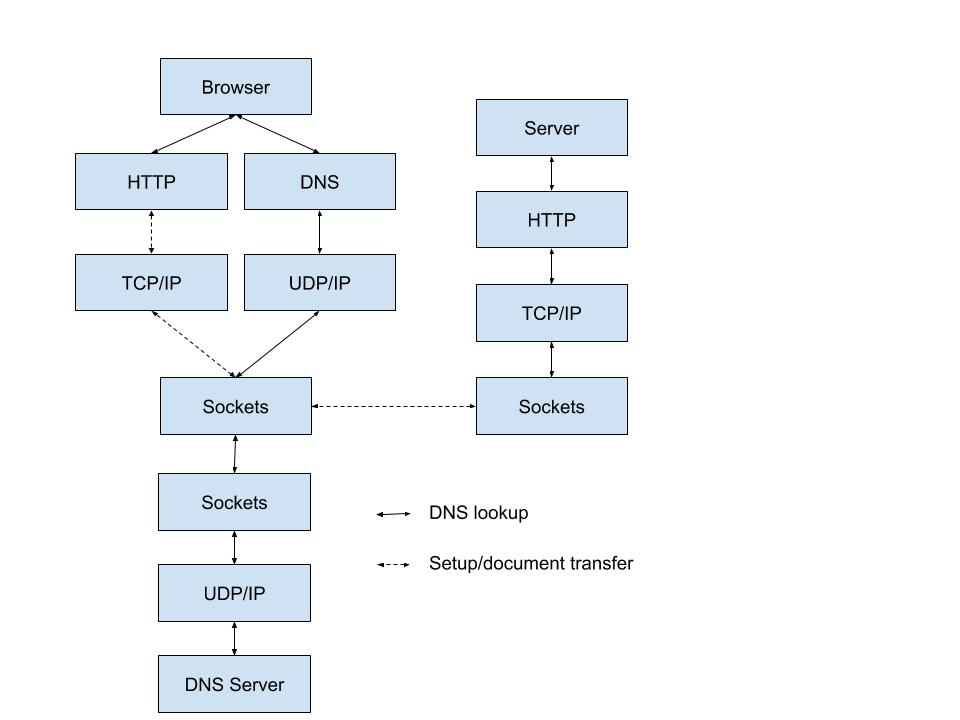
\includegraphics[scale=0.5]{HTTPlayers}
\end{sloppypar}

\begin{sloppypar}
    The requests sent to other microservices throught the network are extremely 
    slow when compared to operation within one computer as the function calls 
    would be. Therefore, the communication patterns should be changed to take 
    into account the change in communication path.
\end{sloppypar}

\begin{sloppypar}
    If the architecture is changed in such a way that the previous communication 
    model amongs the components is preserved, there would be an excessive amount 
    of communication and the resulting system is not as performant as it could 
    be \citep{fowlerlewisms}.
\end{sloppypar}



\section{Confidentiality}
\begin{sloppypar}
    Confidentiality in a web service is usually critical security feature. 
    There are specific services which do not nead information confidentiality 
    regarding some of the data such as public weather services and other similar data.
    Some of the information is still regarded sensitive and must be kept confidential. 
    These data can consists of personal, user, logs or other similar content.
    Users should not be able to use or view content not authorized to him/her. 
    To verify this a form of access control has to be performed. Access control 
    consists of user authentication and authorization. A user has to 
    authenticate him/her self and authorization is acquired to access to 
    information or property.
\end{sloppypar}

\begin{sloppypar}
    In an MA access control can be implemented using sessions. 
    A user authenticates using appropriate channels and a session with a session key is created. 
    The session can have an expiration time and the messages originating from 
    the user interface (UI) carry this key. Sessions and session keys can be used 
    in a distributed system which MSA is but the implementation is more difficult \citep{authinmsa}.
\end{sloppypar}

\subsection{Authentication}
\begin{sloppypar}
    In these cases where the user has to be authenticated the web service needs 
    a way to do this securily. Usually authentication is done using a tuple 
    containing user credentials i.e. a username and a password for the user. The
    user is authenticated and a key or token is transmitted to the user via the 
    network. This communication should in both MA and MSA be encrypted in a way 
    that none of the actors in the transfer path can intercept the message and 
    be able to use the credentials.
\end{sloppypar}

\begin{sloppypar}
    The credential counterparts i.e. shared secret by the server and the user 
    have to be available for the web service for verification. When using MSA 
    the service should own it's own data. When ever such information is 
    available it is a target for thieves and hackers. The services in MSA are 
    to be individually deployable and the service scalable. Authentication 
    service implementation has to take this into account. The service has to 
    adhere to practices that minimize the risks of data breaches. 
\end{sloppypar}
    
\subsubsection{Attacks}
\begin{sloppypar}
    Authentication can be attacked by a multitude of methods.     
    \begin{itemize}
        \item Cracking
        \item Impersonation attacks
        \item Hacking the system
        \item Malware
        \item Social engineering
        \item Cracking the encryption on the communication channel exchanging credentials and keys or tokens.
    \end{itemize}
\end{sloppypar}

\begin{sloppypar}
    From 2013 onwards malware and data breaches performed by hackers have 
    increased and the scale of the damage is massive. The user data containing 
    also the user passwords or hash thereof is valuable commodity which can be 
    traded in the black markets. The damage of the dataloss can be susbtantial. 
    The estimated value from the Yahoo data breach is over \$440 billion. The 
    attacks seem to have been targeted to entities with valuable data and 
    also to such targets that are lacking secure infrastructure. The least likely 
    target to be hacked where non profit organisations and the most likely were 
    medical related organizations \citep{breach}.
\end{sloppypar}
\begin{sloppypar}
    The hacked account credentials have to some extent been available for download 
    from the web. \citet{pwned} created a service where everyone can verify 
    whether any of their accounts are amogst the ones added to the service. 
    The service named as "';-- have i been pwned ?" allows users to enter their 
    username or password to the site and see a result.
\end{sloppypar}

\subsection{Authorization}
\begin{sloppypar}
    Authorization of the user rights can be implemented in various ways. One of 
    which is an authorization service which can contain the access control 
    matrix. Services being accessed verify from the authorization service that
    a particular user or the role that the user has can access the requested 
    service or functionality.
\end{sloppypar}

\begin{sloppypar}
    In a MA the access rights to a functionality can be implemented using
    annotations within the source code. This can be effective since the 
    verification can be done in memory or atleast without network communication. 
    If a session is used it can contain the information needed to verify access 
    rights.
\end{sloppypar}

\begin{sloppypar}
    In contrast to the MA in the MSA the access control matrix or matrices can't 
    be as easily accessed. In order to verify that a specific right exists the 
    service would have communicate with the authorization service every time a user
    tries to access a functionality with access restrictions. This could 
    potentially lead to an extremely lively communication from all the services 
    a formation of a bottleneck to the service.
\end{sloppypar}

https://techbeacon.com/security/microservices-apps-do-identity-access-management-without-overhead



\subsection{Interaction Paradigms}
\begin{sloppypar}
    As already discussed in an MA the service components can communicate using 
    events, procedure calls or other methods available within a single server 
    machine. Usually all this communication stays within a single computer and 
    thus does not necessarily compromise confidentiality.
\end{sloppypar}
\begin{sloppypar}
    In MSA single services communicate via a network.
    
    Next messaging systems list is from \citep{secchalmsa}:
lightweight
-
    REST API,
    Sync RPC,
    GraphQl
    -
    Async REST,
    gRPC
    - 
    Apache Kafka,
    ZeroMQ
    -
    Java Message Service:
    1 ActiveMQ,
    2 JBOSS messaging,
    3 Glassfish
    -
    AMQP:
    1 RabbitMQ,
    2 Qpid,
    3 HornetQ
    -
    MuleESB,
    Apache ServiceMix,
    JBossESB


-
heavyweight

    WebSocket
    



\end{sloppypar}




\subsubsection{Representational State Transfer (REST)}
\begin{sloppypar}
    \citet{restroy} presented REST in 2000 and it has become very successfull. 
    The architecture was derived using various constraints to an architecture.
    One of which is the demand of stateless communication. The communication i.e. 
    the request must contain all information for the server to fullfil the request. 
    All session state is stored in the client and not on the server.
\end{sloppypar}
\begin{sloppypar}
    In her doctoral thesis \citet{secchalmsa} critiques the REST paradigm from 
    the security perspective. She states that the design of the architecture 
    does not meet the security requirements for web applications. The 
    statelessness of REST does not allow for any server side sessions and thus 
    making e.g. token repudiation impossible due to not being able to verify 
    tokens other than the correct issuer by signature and the validity. As such 
    tokens are more compatible with REST but there still has to be the private 
    keys in the server for signature verification.
\end{sloppypar}




\subsubsection{Event-Driven Communication}
\begin{sloppypar}
    
\end{sloppypar}




\subsubsection{Effects on Confidentiality}
\begin{sloppypar}
    
\end{sloppypar}




\subsubsection{Example case}
\begin{sloppypar}
    
\end{sloppypar}




\section{Integrity}
\begin{sloppypar}
    Information integrity in an MA web service is usually left to a single database 
    and sound architectural choices (REALLY? SOURCE).
    Transactions can be used when updating database constents to make sure that
    atomicity, consistency, isolation, and durability (ACID) \citep{acid} is followed.
    When using MSA according to the definition each of the micro services should contain 
    or have access to it's own data i.e. database. This leads to extreme difficulties in information integrity.
    TODO
\end{sloppypar}


\subsection{Introduction}
\subsection{Effects on Integrity}
\subsection{Example case}



\section{Availability}
\begin{sloppypar}
    Availability in this web service context is defined as such that the property or information 
    is available when it is needed.

    
    
\end{sloppypar}

\subsection{Possible Attacks}
\begin{sloppypar}
    D-o-S 
\end{sloppypar}



\subsection{Comparison}
\begin{sloppypar}
    
\end{sloppypar}


\subsection{Introduction}
\begin{sloppypar}

\end{sloppypar}

\subsection{Effects on Availability}
\begin{sloppypar}

\end{sloppypar}

\subsection{Example case}
\begin{sloppypar}

\end{sloppypar}




\section{Other MSA specific security matters}
\subsection{Platforms}
\begin{sloppypar}

\end{sloppypar}

Docker Swarm
Kubernetes (K8s)
Azure

sandbox
virtualization 

\subsection{Monitoring and logging}

\subsection{Software Development}
\subsection{Deployment}
\begin{sloppypar}
    Developing software using the MA the structure the whole application or service 
    is usually deployed as a whole and the program code can be compiled, tested 
    and used as a single unit or multiple modules. In contrast to this a service 
    implemented by using a MSA can be deployed in single microservice units and 
    thus a single service can be worked upon individually and deployed once ready.
\end{sloppypar}

\subsection{Service discovery}
\begin{sloppypar}
    The MSA can have a service discovery service into which all available services 
    can register them selves.

    https://www.nginx.com/blog/service-discovery-in-a-microservices-architecture/

    https://www.consul.io


\end{sloppypar}

\subsection{Externalized configuration}
\begin{sloppypar}
    To allow for easy configuration change management there should exist a 
    configuration orchestration service. This service should have an API from 
    which services in their startup can load their appropriate configuration. 
    The configuration of the whole system can be easily maintained through the 
    API.

    The contents of the configuration is highly sensitive information. It 
    consists of addressess, credentials and other information that alter 
    the behaviour of the system. Therefore, the content must be stored safely 
    and not allowed to be read or altered by unauthorized users.
\end{sloppypar}




% --------------------------------------------------------------------
% --------------------------------------------------------------------

\section{Conclusion}

% Loppuluku päättää työn. Luvun nimi on tyypillisesti ``yhteenveto'' tai
% ``johtopäätöksiä''. Valitse se otsikko, joka tuntuu sopivammalta työsi
% luonteeseen. Joka tapauksessa loppuluku sisältää niin työn yhteenvedon
% kuin johtopäätöksiä työn tulosten perusteella. Pääajatus on antaa
% lukijalle selvä kuva siitä, miten johdannossa asetettuihin
% tavoitteisiin työssä vastattiin.

% Käsittele loppupuvussa seuraavia asioita (jotakuinkin tässä järjestyksessä):
% %
% \begin{itemize}
%   \item Muistutus työn tavoitteista (sidoksisuus johdantoon)
%   \item Päätulokset kootaan yhteen, pohditaan niiden merkitystä
%   \item Suositukset konkreettisiksi toimenpiteiksi (``Mitä sitten?'' 
% Nyt kun käytössä on tämän työn myötä tullut tieto, 
% mitä se nyt tarkoittaa tälle asialle/alalle.)
%   \item Tulosten soveltuvuus, käyttöön liittyvät rajoitukset
%   \item Jatkotutkimustarve 
% (``Tulevaisuudessa olisi mielenkiintoista selvittää...'' tms.)
%   \item Työn onnistumisen arviointi 
% (Huom! Älä arvioi omaa kirjoitusprosessiasi vaan tekemääsi tutkimusta)
% \end{itemize}

% --------------------------------------------------------------------

